% Informe Final de Gestión · FinBank · Corte 3
% Fuente editable. Se compila con: python scripts/build_corte3.py
% Las tablas y cifras vienen de generated/ (producidas desde docs/corte3/data y el código).
\documentclass[10pt,a4paper]{article}
\usepackage[T1]{fontenc}
\usepackage[utf8]{inputenc}
\usepackage{lmodern}
\usepackage[spanish,es-noshorthands,es-tabla]{babel}
\usepackage[a4paper,margin=2.1cm,headheight=14pt]{geometry}
\usepackage{booktabs,tabularx,array,graphicx,xcolor,fancyhdr,titlesec,enumitem,caption,microtype}
\usepackage[hyphens]{url}
\usepackage[hidelinks]{hyperref}
\usepackage{tcolorbox}
\usepackage{amsmath}

\definecolor{navy}{HTML}{1F3A5F}
\definecolor{teal}{HTML}{2A9D8F}
\definecolor{amber}{HTML}{E9A23B}
\definecolor{rojo}{HTML}{C8553D}
\definecolor{gris}{HTML}{6B7280}
\hypersetup{colorlinks=true,linkcolor=navy,urlcolor=teal}

\newcommand{\VelMedia}{15,2}
\newcommand{\VelMediaTotal}{14,67}
\newcommand{\PuntosTotal}{88}
\newcommand{\SseisComp}{15}
\newcommand{\SseisDone}{12}
\newcommand{\SseisPend}{3}
\newcommand{\Throughput}{4}
\newcommand{\CicloMedio}{5,25}
\newcommand{\DiasBloqueo}{3}
\newcommand{\WIPMax}{3}
\newcommand{\BaseTotal}{169,2}
\newcommand{\GastoTotal}{169,0}
\newcommand{\DesvCosto}{-0,12 \%}
\newcommand{\DesvSdos}{-2,84 \%}
\newcommand{\GastoSdos}{54,8}
\newcommand{\BaseSdos}{56,4}
\newcommand{\EACSseis}{169,5}
\newcommand{\DesvScinco}{0,21 \%}
\newcommand{\NoEjecutado}{11,0}
\newcommand{\Reserva}{10,8}
\newcommand{\Autorizado}{180}
\newcommand{\AUCtreinta}{0,7959}
\newcommand{\AUCsesenta}{0,7884}
\newcommand{\AUCchurn}{0,7673}
\newcommand{\RecallOp}{0,6203}
\newcommand{\RecallCosto}{0,4094}
\newcommand{\PrecOp}{0,2232}
\newcommand{\PrecCosto}{0,3102}
\newcommand{\CorteOp}{0,13}
\newcommand{\CorteCosto}{0,21}
\newcommand{\CorteMora}{0,09}
\newcommand{\BenefOp}{11,55}
\newcommand{\BenefCosto}{20,05}
\newcommand{\BenefDif}{8,51}
\newcommand{\MuestraOOT}{4.691}
\newcommand{\TasaMora}{5,65 \%}
\newcommand{\TasaChurn}{10,08 \%}
\newcommand{\EWTotal}{1.356}
\newcommand{\EWFlag}{250}
\newcommand{\ChurnTotal}{1.062}
\newcommand{\ChurnFlag}{319}
\newcommand{\SemAlerta}{4}
\newcommand{\SemReentreno}{5}
\newcommand{\PSIbureau}{0,396}
\newcommand{\AUCbase}{0,794}
\newcommand{\AUCsemReentreno}{0,648}
\newcommand{\Tests}{57}
\newcommand{\SHA}{d873b15}
\newcommand{\Rama}{c3/s6/s6-05-cierre}
\newcommand{\Generado}{2026-11-18 04:45 UTC}
\newcommand{\PyVer}{3.11.9}

\newcommand{\repo}{\href{https://github.com/OscarSantiagoMerino/DataForge-Consulting}{OscarSantiagoMerino/DataForge-Consulting}}
\newcommand{\rot}[1]{\textsf{\scriptsize\color{gris}[#1]}}

\titleformat{\section}{\large\bfseries\color{navy}}{\thesection.}{0.5em}{}
\titleformat{\subsection}{\normalsize\bfseries\color{navy}}{\thesubsection}{0.5em}{}
\titlespacing*{\section}{0pt}{1.2em}{0.5em}
\titlespacing*{\subsection}{0pt}{0.8em}{0.3em}
\setlist{nosep,leftmargin=1.3em}
\captionsetup{font=small,labelfont={bf,color=navy}}
\setlength{\parskip}{0.45em}
\setlength{\parindent}{0pt}
\renewcommand{\arraystretch}{1.15}

\pagestyle{fancy}
\fancyhf{}
\lhead{\small\color{gris}Informe Final de Gestión · FinBank S.A.}
\rhead{\small\color{gris}DataForge Consulting · GMAC-FB-2026-01}
\cfoot{\small\thepage}
\renewcommand{\headrulewidth}{0.3pt}

\begin{document}

% ------------------------------------------------------------------ portada
\begin{titlepage}
\color{navy}
\vspace*{1.2cm}
{\large DataForge Consulting}\\[0.3em]
{\color{gris}\rule{\linewidth}{0.6pt}}\\[1.5cm]
{\fontsize{30}{36}\selectfont\bfseries Informe Final de Gestión}\\[0.6cm]
{\Large Programa de Analítica Predictiva:\\ mora temprana y churn de crédito}\\[1.2cm]
\color{black}
\begin{tabular}{@{}ll}
Cliente & FinBank S.A., Vicepresidencia de Riesgo y Analítica \\
Código del proyecto & GMAC-FB-2026-01 \\
Cierre del escenario & Sprint 6, semanas 11--12 (19--30 de octubre de 2026) \\
Entrega académica & 18 de noviembre de 2026 · Sustentación: 20 de noviembre de 2026 \\
Grupo & Grupo X (número por confirmar) \\
\end{tabular}

\vspace{1.2cm}
\begin{tabular}{@{}lll}
\textbf{Integrante} & \textbf{Rol en el Charter} & \textbf{Rol Scrum (Corte 2 y 3)} \\
\midrule
Daniel Felipe Martínez Hernández & Líder de proyecto & Developer; reporte formal al patrocinador \\
Rafael Alejandro Baracaldo Doikov & Analista de negocio & Product Owner y Developer \\
Oscar Santiago Merino Suárez & Facilitador Scrum & Scrum Master y Developer \\
\end{tabular}

\vfill
\begin{tcolorbox}[colback=navy!4,colframe=navy!40,boxrule=0.4pt,arc=1mm,left=2mm,right=2mm]
\small\textbf{Cómo leer las cifras.} Cada dato lleva su origen.
\rot{Base} línea base del Charter.
\rot{Antecedente} escenario de los Cortes 1 y 2 (S1--S2).
\rot{Reconstrucción C3} transición S3--S5 reconstruida en este corte.
\rot{Simulación C3} hechos simulados del Sprint 6.
\rot{Verificable} resultado técnico del repositorio, que cualquiera puede reproducir.
Los actos de aceptación reales (firma del patrocinador, Finanzas, oficial de protección de datos, aprobaciones en GitHub) se registran aparte y \textbf{no} se simulan.
\end{tcolorbox}
\vspace{0.4cm}
{\small Escuela Colombiana de Ingeniería Julio Garavito · Gestión de Métodos Ágiles y Clásicos (GMAC) · Corte 3}
\end{titlepage}

% ------------------------------------------------------------------ 1
\section{Resumen ejecutivo}

\textbf{La decisión que pedimos a FinBank es cerrar el programa con transferencia condicionada.} En doce semanas y dentro del sobre autorizado, DataForge entregó los dos modelos que el Charter compromete (mora a 30/60 días y churn a tres meses), una regla de decisión con su matriz de costos, un piloto operando sobre un segmento controlado, un plan de monitoreo con disparador de reentrenamiento y el marco de gestión (tablero, backlog, Definition of Done y runbook) para que FinBank lo opere sin el consultor. Falta un acto que no depende del equipo: la firma del acta de entrega, condicionada a que el oficial de protección de datos cierre un hallazgo sobre la sal de seudonimización.

\begin{itemize}
\item \textbf{Alcance.} \PuntosTotal{} puntos terminados en seis sprints, con velocidad media de \VelMedia{} puntos en S1--S5. El Sprint 6 comprometió \SseisComp{} puntos y cerró \SseisDone{}. Los \SseisPend{} restantes son S6-04, que espera la firma del acta. \rot{Simulación C3}
\item \textbf{Costo.} Se gastaron COP \GastoTotal{} millones frente a una base de \BaseTotal{} millones, con una desviación de \DesvCosto{}, dentro del límite del 5\,\% (O5). La reserva de COP \Reserva{} millones no se liberó. \rot{Simulación C3}
\item \textbf{Cronograma.} El hito final se alcanzó en la semana 12. M2 llegó 3 semanas tarde y M4, 1 semana, ambos por la dependencia del extracto de churn. \rot{Reconstrucción C3}
\item \textbf{Modelos.} Sobre datos sintéticos, el prototipo del repositorio obtiene un AUC fuera de tiempo de \AUCtreinta{} (30 días) y un recall de churn de \RecallOp{} al umbral operativo, por encima de las metas del Charter (0,75 y 0,60). \rot{Verificable} La validación con datos de FinBank queda pendiente.
\item \textbf{Decisión abierta para Finanzas.} El umbral de máximo beneficio en churn (\CorteCosto) da un recall de \RecallCosto{} e incumple O2. Cumplir O2 con el umbral \CorteOp{} reduce el beneficio neto en COP \BenefDif{} millones en la cohorte sintética. Proponemos priorizar O2 y que Finanzas ratifique la regla.
\end{itemize}

% ------------------------------------------------------------------ 2
\section{Problema, alcance y objetivos}

FinBank administra una cartera de COP 420.000 millones con 125.000 clientes. Registra la mora cuando el pago ya se perdió y la cancelación cuando el cliente ya se fue. El Charter estima la exposición en COP 58.800 millones por mora temprana sin alerta y en COP 18.200 millones por churn no anticipado del segmento preferencial, unos COP 77.000 millones en total, cerca del 18\,\% de la cartera \rot{Base}. El diagnóstico concluyó que el obstáculo no son los datos ni los analistas: falta una forma definida de planear, controlar y cerrar proyectos analíticos.

El alcance incluye la gestión del proyecto, el diagnóstico de datos, los dos modelos, el análisis de umbrales y un piloto controlado con monitoreo y capacitación. Quedan fuera la infraestructura de core bancario o CRM, la ejecución de campañas de retención, otros productos y la migración de historia anterior a 36 meses. La línea base es fija: 12 semanas, seis sprints de dos semanas, COP 180.000.000 autorizados (169,2 millones por rubros y 10,8 de reserva) y una desviación máxima del 5\,\% \rot{Base}.

\begin{table}[h]
\caption{Trazabilidad de los objetivos del Charter al cierre}\label{tab:obj}
\footnotesize
\begin{tabularx}{\linewidth}{l X X p{3.4cm}}
\toprule
\textbf{Obj.} & \textbf{Medida de éxito (Charter)} & \textbf{Resultado en el escenario / prototipo} & \textbf{Estado real} \\
\midrule
O1 & AUC $\geq$ 0,75 fuera de tiempo & Cumple en el prototipo: 0,7959 (30 d), 0,7884 (60 d) & Pendiente con datos reales \\
O2 & Recall $\geq$ 0,60 al umbral operativo & Cumple en el prototipo: 0,6203 al umbral 0,13 & Pendiente con datos reales \\
O3 & Matriz de costos y umbral aprobados por Finanzas & Aprobado en el escenario (Review S5) & Pendiente: aprobación real de Finanzas \\
O4 & Aceptación del paquete de transferencia por el patrocinador & Condicionada (Review S6) & Pendiente: firma real \\
O5 & Desviación de costo y cronograma $\leq$ 5 \% & Cumple: costo -0,12 \%, hito final en la semana 12 & Cifras del escenario; sin registro contable real \\
\bottomrule
\end{tabularx}

\end{table}

% ------------------------------------------------------------------ 3
\section{Trayectoria del programa: S1 a S6}

\begin{table}[h]
\caption{Cierre de los seis sprints (compromiso y puntos que cumplen la DoD)}\label{tab:sprints}
\footnotesize
\begin{tabularx}{\linewidth}{l c X r r r l l}
\toprule
\textbf{Sprint} & \textbf{Sem.} & \textbf{Objetivo del sprint} & \textbf{Comp.} & \textbf{Hecho} & \textbf{Cumpl.} & \textbf{Meta} & \textbf{Rótulo} \\
\midrule
S1 & 1-2 & El proyecto queda gobernado y el equipo puede tocar datos legalmente & 16 & 16 & 100\,\% & Cumplida & Antecedente \\
S2 & 3-4 & Base de datos validada para los modelos de mora y churn & 20 & 15 & 75\,\% & Parcial & Antecedente \\
S3 & 5-6 & Modelo de mora a 30/60 días validado fuera de tiempo (M3) & 16 & 16 & 100\,\% & Cumplida & Reconstrucción C3 \\
S4 & 7-8 & Extracto de churn integrado y modelo de churn construido (M2 y M4) & 16 & 13 & 81\,\% & Parcial & Reconstrucción C3 \\
S5 & 9-10 & Churn validado y reglas de decisión aprobadas por Finanzas (M4 y M5) & 16 & 16 & 100\,\% & Cumplida & Reconstrucción C3 \\
S6 & 11-12 & Piloto operando en el segmento controlado y paquete de transferencia listo para firma (M6) & 15 & 12 & 80\,\% & Parcial & Simulación C3 \\
\bottomrule
\end{tabularx}

\end{table}

\textbf{S1--S2, antecedente.} S1 cerró 16 de 16 puntos: Charter, acuerdo de acceso bajo la Ley 1581, perfilamiento sobre la muestra anonimizada y tablero con DoD. S2 comprometió 20 puntos y cerró 15. El extracto de churn (T-05.5, 5 puntos) dependía de una credencial del área de TI que no llegó. El equipo lo pasó a Blocked el día 6, el Scrum Master escaló al día siguiente y el Product Owner adelantó la variable objetivo de mora. Al cierre de S2 el gasto era COP \GastoSdos{} millones frente a \BaseSdos{} planeados (\DesvSdos) y M2 no cerró porque el diccionario no tenía variables de churn \rot{Antecedente}.

\textbf{S3--S5, reconstrucción.} El pronóstico del Corte 2 fijó S3 en 16 puntos como máximo. La retrospectiva de S2 añadió una Definition of Ready: ningún ítem con una dependencia externa sin conceder entra al sprint. La credencial llegó el día 2 de S3, \emph{después} de la Planning, así que T-05.5 no entró en S3. El sprint se dedicó al modelo de mora (US-06, 13 puntos) y al diseño de la validación fuera de tiempo, y M3 cerró en la semana 6. En S4 se integró el extracto, se añadieron las variables de churn al diccionario (M2 cerró en la semana 7) y se construyó el modelo de churn. Su validación (US-08b) necesitaba que madurara la ventana de tres meses, lo que ocurrió en la semana 9, y pasó a S5: M4 se desplazó una semana. \textbf{Ningún trabajo de churn se dio por terminado antes de tener el extracto.} S5 cerró la validación de churn, la calibración y la matriz de costos con Finanzas (M5, semana 10) \rot{Reconstrucción C3}.

\begin{table}[h]
\caption{Backlog de S3--S5 y su vínculo con objetivos e hitos}\label{tab:trace}
\footnotesize
\begin{tabularx}{\linewidth}{l l X r l l l}
\toprule
\textbf{Sprint} & \textbf{ID} & \textbf{Ítem} & \textbf{Pts} & \textbf{Obj.} & \textbf{Hito} & \textbf{Estado} \\
\midrule
S3 & T-06.1 & Diseño de la validación fuera de tiempo & 3 & O1 & M3 & Done \\
S3 & US-06 & Modelo de mora a 30 y 60 días & 13 & O1 & M3 & Done \\
S4 & T-05.5 & Extracto histórico de churn & 5 & O2 & M2 & Done \\
S4 & T-08.1 & Variables de churn en el diccionario & 3 & O2 & M2 & Done \\
S4 & US-08a & Modelo de churn a 3 meses: construcción & 5 & O2 & M4 & Done \\
S4 & US-08b & Modelo de churn: validación fuera de tiempo y recall al umbral & 3 & O2 & M4 & No terminado (pasa a S5) \\
S5 & US-08b & Modelo de churn: validación fuera de tiempo y recall al umbral & 3 & O2 & M4 & Done \\
S5 & T-09.1 & Calibración de probabilidades & 5 & O3 & M5 & Done \\
S5 & US-09 & Matriz de costos y umbrales con Finanzas & 8 & O3 & M5 & Done \\
\bottomrule
\end{tabularx}

\end{table}

% ------------------------------------------------------------------ 4
\section{Sprint 6: el sprint final}

\textbf{Objetivo.} \emph{El piloto opera en el segmento controlado y el paquete de transferencia queda listo para la firma del patrocinador (M6).}

\textbf{Capacidad razonada.} La velocidad media de S1--S5 fue \VelMedia{} puntos. Siguiendo la regla de la retrospectiva de S2 (no comprometer más que la velocidad media), el equipo comprometió 15 puntos. Las dependencias externas conocidas (ambiente de piloto de TI y auditoría del oficial de protección de datos) se registraron en la Planning. El compromiso se publicó en GitHub como issues \#10--\#14 antes de empezar el trabajo técnico.

\begin{table}[h]
\caption{Sprint Backlog de S6 (cada historia tiene criterios Dado/Cuando/Entonces y DoD en su issue)}\label{tab:s6}
\scriptsize
\begin{tabularx}{\linewidth}{l X r p{1.5cm} p{1.7cm} p{2.3cm} p{1.1cm} l p{1.9cm}}
\toprule
\textbf{ID} & \textbf{Historia} & \textbf{Pts} & \textbf{Resp.} & \textbf{Negocio} & \textbf{Dependencia} & \textbf{Obj.} & \textbf{Issue} & \textbf{Estado (escenario)} \\
\midrule
S6-01 & Piloto controlado con lista semanal de alerta temprana (incluye US-07) & 5 & Rafael y Oscar & Cobranza & ambiente de piloto de TI & O1 O2 O3 O4 & \#10 & Done \\
S6-02 & Monitoreo de desempeño y drift & 3 & Oscar & Riesgo y Analítica & S6-01 & O4 & \#11 & Done \\
S6-03 & Runbook de operación del piloto & 2 & Daniel & Riesgo y Analítica & S6-01 & O4 & \#12 & Done \\
S6-04 & Paquete de transferencia y capacitación & 3 & Rafael & Patrocinador & auditoría del oficial de protección de datos & O4 & \#13 & No terminado (firma pendiente) \\
S6-05 & Balance final de cronograma y presupuesto & 2 & Daniel & Finanzas & registro de gasto S1-S6 & O5 & \#14 & Done \\
\bottomrule
\end{tabularx}

\end{table}

\textbf{Definition of Done.} Reproducible desde el repositorio, documentada, pruebas en verde en CI, PR aprobado por un integrante distinto del autor, validada por el responsable de negocio y demostrada en la Sprint Review.

\subsection{Daily Scrum: los días en que cambió el plan}
\scriptsize
\begin{tabularx}{\linewidth}{l l l l X}
\toprule
\textbf{Día} & \textbf{Fecha (esc.)} & \textbf{Tipo} & \textbf{Ítem} & \textbf{Registro (simulado)} \\
\midrule
D1 & 19 oct 2026 & Planning &  & Sprint Planning: objetivo del sprint y compromiso de 5 historias y 15 puntos (velocidad media S1-S5 = 15,2). WIP máximo 3 en In Progress. \\
D1 & 19 oct 2026 & Avance & S6-01 & Pairing: Rafael conduce y Oscar navega. Modelo de mora y listas sobre la cohorte de desarrollo. \\
D1 & 19 oct 2026 & Avance & S6-03 & Borrador del runbook a partir de los comandos del pipeline. \\
D2 & 20 oct 2026 & Avance & S6-01 & Listas con identificador seudonimizado; falta correr en el ambiente de piloto de TI. \\
D3 & 21 oct 2026 & Bloqueo & S6-01 & El ambiente de piloto no tiene la cuenta de servicio. S6-01 pasa a Blocked con la causa escrita. \\
D3 & 21 oct 2026 & Cambio de plan & S6-02 & El Product Owner adelanta el monitoreo (S6-02) para no dejar capacidad ociosa. \\
D4 & 22 oct 2026 & Escalación & S6-01 & El Scrum Master escala al patrocinador dentro de las 24 horas (regla de la retrospectiva de S2). La demo sigue sobre la réplica sintética del repositorio. \\
D4 & 22 oct 2026 & Done & S6-03 & Runbook terminado y revisado por un par: 2 puntos. \\
D5 & 23 oct 2026 & Cambio de alcance & US-10 & Retención pide variables explicativas por cliente en la lista de churn. Entra al Product Backlog como US-10 y no al sprint (riesgo R6). \\
D5 & 23 oct 2026 & Avance & S6-05 & Consolidación del registro de gasto S1-S6. \\
D6 & 26 oct 2026 & Desbloqueo & S6-01 & TI habilita el ambiente de piloto tras 3 días de bloqueo (D3-D5). \\
D6 & 26 oct 2026 & Done & S6-02 & Monitoreo con PSI y disparador de reentrenamiento: 3 puntos. \\
D7 & 27 oct 2026 & Avance & S6-01 & Primera corrida en el segmento controlado; Cobranza revisa la lista. \\
D7 & 27 oct 2026 & Avance & S6-04 & Inicio del paquete de transferencia; WIP en 3 (S6-01 S6-04 S6-05). \\
D8 & 28 oct 2026 & Done & S6-01 & Cobranza valida la lista contra su proceso operativo: 5 puntos. \\
D8 & 28 oct 2026 & Avance & S6-04 & Sesiones de capacitación 1 y 2 con analistas de Riesgo y TI. \\
D9 & 29 oct 2026 & Done & S6-05 & Balance final presentado a Finanzas: desviación de costo -0,12 \%: 2 puntos. \\
D10 & 30 oct 2026 & Bloqueo & S6-04 & Auditoría del oficial de protección de datos: el piloto usa la sal de demostración. Exige una sal propia bajo su custodia antes de firmar. S6-04 queda fuera de Done. \\
D10 & 30 oct 2026 & Review &  & Sprint Review con demo del piloto y del monitoreo. Decisión del patrocinador: cierre con transferencia condicionada. \\
D10 & 30 oct 2026 & Retrospectiva &  & Retrospectiva de cierre del proyecto con acciones y responsable. \\
\bottomrule
\end{tabularx}


\subsection{Sprint Review y aceptación por criterio}
En la Review del día 10 \rot{Simulación C3} se demostraron el piloto (lista semanal de alerta y lista de churn) y el monitoreo. El patrocinador aceptó S6-01, S6-02, S6-03 y S6-05. S6-04 quedó fuera de Done por el hallazgo de la auditoría de protección de datos. La tabla \ref{tab:acc6} separa lo que se cumple en el escenario de la evidencia técnica que lo respalda. El registro completo, con el estado real de cada criterio y quién puede resolverlo, está en el Anexo A.

\begin{table}[h]
\caption{Aceptación de las historias de S6 por criterio}\label{tab:acc6}
\scriptsize
\begin{tabularx}{\linewidth}{l X p{3cm} X}
\toprule
\textbf{Historia} & \textbf{Criterio de aceptación} & \textbf{Escenario} & \textbf{Evidencia técnica} \\
\midrule
S6-01 & Lista semanal seudonimizada sin columnas personales & Cumple (S6 D8) & test\_\allowbreak{}lists\_\allowbreak{}carry\_\allowbreak{}no\_\allowbreak{}personal\_\allowbreak{}data\_\allowbreak{}and\_\allowbreak{}only\_\allowbreak{}pseudonymous\_\allowbreak{}keys; PR \#17 \\
S6-01 & Métricas rotuladas como prototipo sintético & Cumple & pilot\_\allowbreak{}metrics.csv; PR \#17 \\
S6-01 & Dos corridas idénticas & Cumple & test\_\allowbreak{}two\_\allowbreak{}runs\_\allowbreak{}give\_\allowbreak{}identical\_\allowbreak{}outputs; hashes de run\_\allowbreak{}pilot.py \\
S6-01 & Validación de Cobranza contra el proceso operativo & Cumple (escenario S6 D8) & — \\
S6-02 & Bandas de PSI estable / vigilar / alerta & Cumple (S6 D6) & test\_\allowbreak{}psi\_\allowbreak{}status\_\allowbreak{}bands; PR \#18 \\
S6-02 & Reentrenamiento tras 2 semanas con caída de AUC o recall > 0,05 & Cumple & Pruebas de rachas de AUC y recall; PR \#18 \\
S6-02 & Detección del cambio inyectado & Cumple & monitoring\_\allowbreak{}report.csv: bureau\_\allowbreak{}score en alerta en semana 4 y reentrenamiento en la 5 \\
S6-03 & Runbook ejecutable en copia limpia & Cumple (S6 D4) & Clon limpio con 6 salidas; PR \#19 \\
S6-03 & Acción, rol y plazo por caso & Cumple & RUNBOOK.md sección 5 \\
S6-04 & Inventario con ubicación y responsable & Cumple & TRANSFERENCIA.md sección 1; PR \#20 \\
S6-04 & Capacitación con registro de asistentes & Cumple (escenario S6 D8) & Plan en TRANSFERENCIA.md sección 2 \\
S6-04 & Acta firmable tras la auditoría de protección de datos & No cumple: hallazgo de la sal (S6 D10) & TRANSFERENCIA.md secciones 4 y 5 \\
S6-05 & Base aprobada, gasto, pronóstico y reserva separados & Cumple (S6 D9) & budget.csv; informe sección 8 \\
S6-05 & Hitos M1-M6 con desviación y evidencia & Cumple & milestones.csv \\
\bottomrule
\end{tabularx}

\end{table}

% ------------------------------------------------------------------ 5
\section{Evidencias del tablero y de GitHub}

\textbf{Tablero.} El token de GitHub de la cuenta no tiene el permiso de \emph{Projects}, así que el tablero del Corte 3 se lleva con etiquetas \texttt{estado:*} sobre las issues (Backlog, Ready, In Progress, Blocked, Review, Done), el milestone \emph{Corte 3 · S6} y una vista reproducible (\texttt{docs/corte3/TABLERO.md}) que genera \texttt{scripts/github\_snapshot.py} desde la API. Reglas: Ready exige la DoR; In Progress tiene WIP máximo de 3; Blocked exige la causa y el responsable en un comentario y escalación en 24 horas; Review empieza al abrir el PR con CI; Done exige el PR fusionado y la DoD completa. El Trello del Corte 1 es el antecedente histórico.

\textbf{Flujo en GitHub} \rot{Verificable}. Cada historia tiene una issue, una rama \texttt{c3/s6/<id>-<tema>} y un PR con alcance, pruebas y criterios. Los PR forman una cadena y deben integrarse en orden con \emph{merge commit}, la regla del Corte 2. El CI corre las pruebas, el pipeline, el piloto y el monitoreo en cada push. La aprobación de cada PR corresponde a un integrante distinto del autor, y las revisiones ya se pidieron. Al generar este informe ningún PR del Corte 3 tenía aprobación ni merge, como muestra la tabla. Esos estados se actualizan con \texttt{github\_snapshot.py} y no se dan por hechos.

\begin{table}[h]
\caption{Bitácora de GitHub del Corte 3 (leída de la API al generar el informe)}\label{tab:gh}
\scriptsize
\begin{tabularx}{\linewidth}{l l l l X l l l}
\toprule
\textbf{ID} & \textbf{Issue} & \textbf{Columna} & \textbf{PR} & \textbf{Rama} & \textbf{CI} & \textbf{Aprobación} & \textbf{Merge} \\
\midrule
S6-01 & \href{https://github.com/OscarSantiagoMerino/DataForge-Consulting/issues/10}{\#10} & done & \href{https://github.com/OscarSantiagoMerino/DataForge-Consulting/pull/17}{\#17} & \texttt{c3/s6/s6-01-piloto} & success & Ch0comilo & 8bd9e3e \\
S6-02 & \href{https://github.com/OscarSantiagoMerino/DataForge-Consulting/issues/11}{\#11} & review & \href{https://github.com/OscarSantiagoMerino/DataForge-Consulting/pull/18}{\#18} & \texttt{c3/s6/s6-02-monitoreo} & success & correoalejandro & cc95ed4 \\
S6-03 & \href{https://github.com/OscarSantiagoMerino/DataForge-Consulting/issues/12}{\#12} & review & \href{https://github.com/OscarSantiagoMerino/DataForge-Consulting/pull/19}{\#19} & \texttt{c3/s6/s6-03-runbook} & success & correoalejandro & 9570e93 \\
S6-04 & \href{https://github.com/OscarSantiagoMerino/DataForge-Consulting/issues/13}{\#13} & blocked & \href{https://github.com/OscarSantiagoMerino/DataForge-Consulting/pull/20}{\#20} & \texttt{c3/s6/s6-04-transferencia} & success & correoalejandro & 4d079a7 \\
S6-05 & \href{https://github.com/OscarSantiagoMerino/DataForge-Consulting/issues/14}{\#14} & review & \href{https://github.com/OscarSantiagoMerino/DataForge-Consulting/pull/21}{\#21} & \texttt{c3/s6/s6-05-cierre} & success & pendiente & pendiente \\
C3-00 & \href{https://github.com/OscarSantiagoMerino/DataForge-Consulting/issues/15}{\#15} & review & \href{https://github.com/OscarSantiagoMerino/DataForge-Consulting/pull/16}{\#16} & \texttt{c3/s6/c3-00-gitignore-videos} & success & Ch0comilo & f0429f2 \\
C3-00 & \href{https://github.com/OscarSantiagoMerino/DataForge-Consulting/issues/15}{\#15} & review & \href{https://github.com/OscarSantiagoMerino/DataForge-Consulting/pull/21}{\#21} & \texttt{c3/s6/s6-05-cierre} & success & pendiente & pendiente \\
C3-01 & \href{https://github.com/OscarSantiagoMerino/DataForge-Consulting/issues/22}{\#22} & review & \href{https://github.com/OscarSantiagoMerino/DataForge-Consulting/pull/23}{\#23} & \texttt{c3/s6/c3-01-sitio-web} & success & pendiente & pendiente \\
\bottomrule
\end{tabularx}

\end{table}

El PR \#9 del Corte 2 sigue abierto y sin aprobación. Se conserva como antecedente. La cadena del Corte 3 parte de \texttt{main} y no modifica los archivos de ese PR (\texttt{README.md} y los documentos de \texttt{docs/}), salvo dos líneas añadidas al final de \texttt{ci.yml} que no se solapan con su cambio.

% ------------------------------------------------------------------ 6
\section{Velocidad, burndown y métricas de flujo}

\begin{figure}[h]
\centering
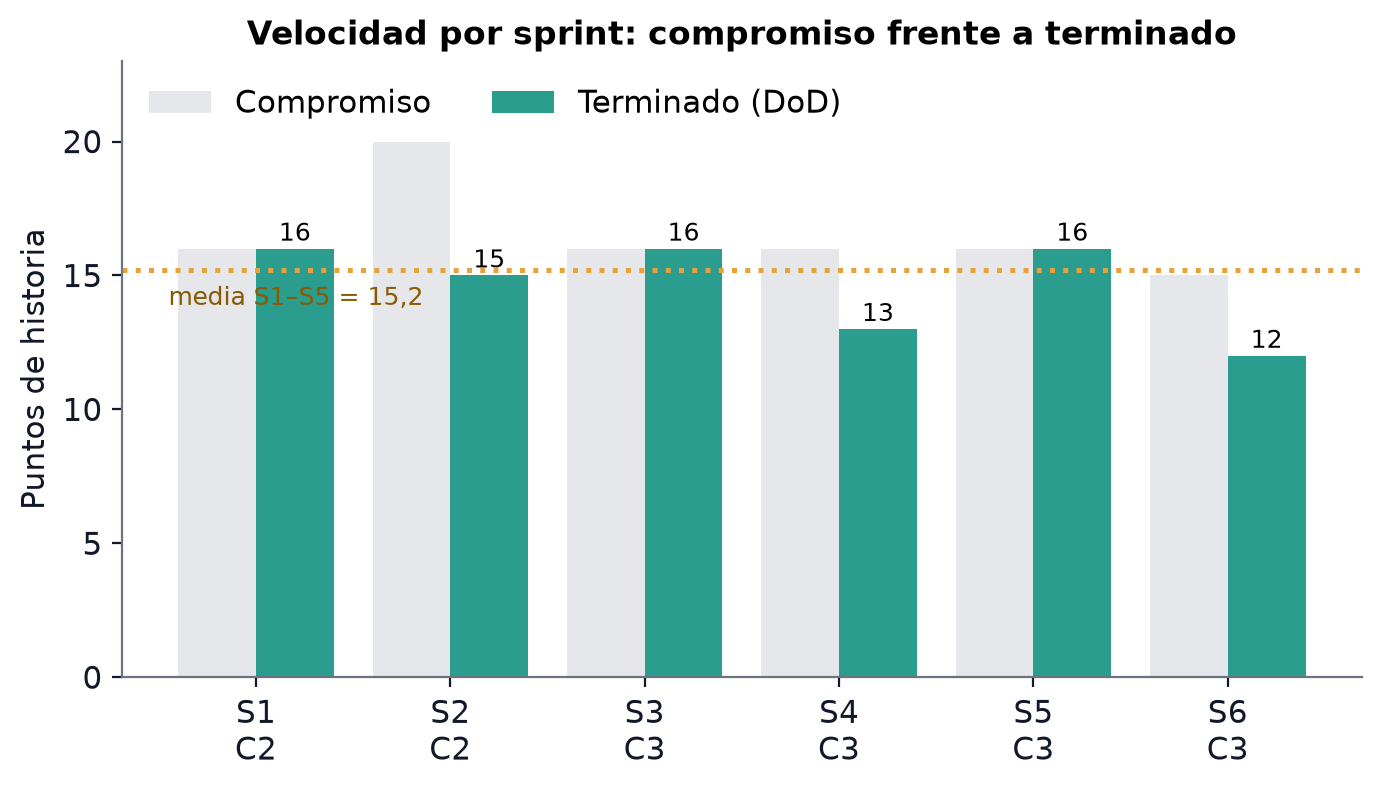
\includegraphics[width=0.49\linewidth]{../figures/velocity.png}\hfill
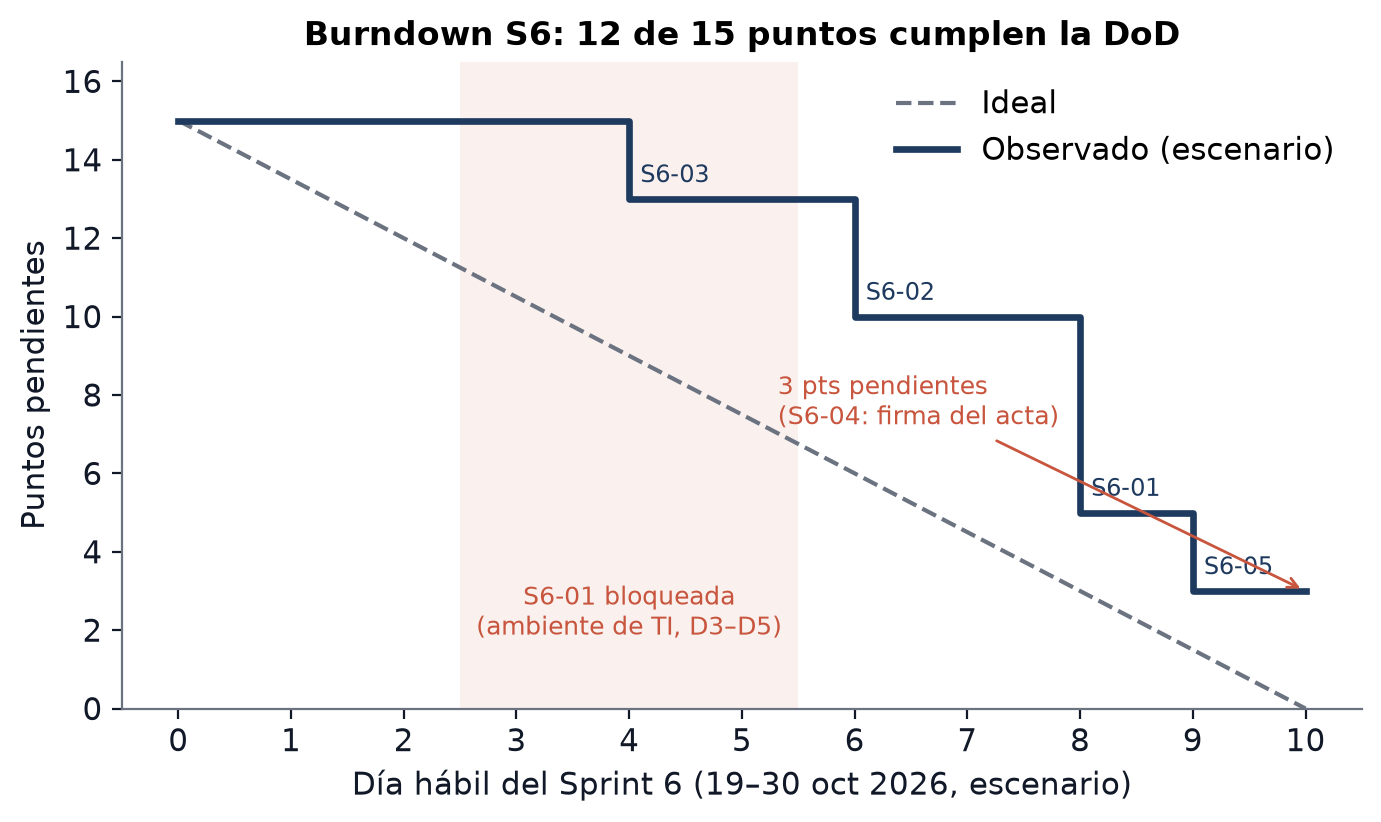
\includegraphics[width=0.49\linewidth]{../figures/burndown_s6.png}
\caption{Velocidad S1--S6 y burndown de S6. Los puntos se descuentan solo el día en que el ítem cumple su DoD en el escenario.}\label{fig:vel}
\end{figure}

La curva de S6 sigue plana hasta el día 4: S6-01 estuvo bloqueada del día 3 al 5 y el Product Owner adelantó S6-02 para no dejar capacidad ociosa. Del día 6 al 9 se recupera, pero cierra con \SseisPend{} puntos pendientes, que corresponden a S6-04. A diferencia de S2, el faltante no viene de comprometer de más: viene de un acto externo (la auditoría) que llegó el último día. La retrospectiva lo convierte en una acción concreta.

\begin{table}[h]
\caption{Métricas de S6. Velocidad, throughput, tiempo de ciclo y WIP se reportan por separado}\label{tab:flow}
\footnotesize
\begin{tabularx}{\linewidth}{l l X}
\toprule
\textbf{Métrica} & \textbf{Valor} & \textbf{Cálculo / nota} \\
\midrule
Velocidad S6 (puntos que cumplen la DoD) & 12 de 15 & Suma de puntos de ítems Done al cierre \\
Velocidad media S1--S5 & 15,2 & Base de la capacidad de S6 \\
Throughput S6 (ítems terminados) & 4 & Conteo de ítems Done \\
Tiempo de ciclo medio & 5,25 días & S6-01: 8, S6-02: 4, S6-03: 4, S6-05: 5 \\
Días bloqueados & 3 & S6-01, D3--D5 (ambiente de TI) \\
WIP máximo en In Progress & 3 (límite 3) & Día 7 \\
Cambios de alcance & 1 (fuera del sprint) & US-10 al Product Backlog (R6) \\
\bottomrule
\end{tabularx}

\end{table}

\footnotesize
\begin{tabularx}{\linewidth}{r r r X r r}
\toprule
\textbf{Día} & \textbf{Ideal} & \textbf{Pendiente} & \textbf{Ítems que cumplen la DoD ese día} & \textbf{WIP} & \textbf{Bloq.} \\
\midrule
0 & 15,0 & 15 & — & 0 & 0 \\
1 & 13,5 & 15 & — & 2 & 0 \\
2 & 12,0 & 15 & — & 2 & 0 \\
3 & 10,5 & 15 & — & 2 & 1 \\
4 & 9,0 & 13 & S6-03 & 1 & 1 \\
5 & 7,5 & 13 & — & 2 & 1 \\
6 & 6,0 & 10 & S6-02 & 2 & 0 \\
7 & 4,5 & 10 & — & 3 & 0 \\
8 & 3,0 & 5 & S6-01 & 2 & 0 \\
9 & 1,5 & 3 & S6-05 & 1 & 0 \\
10 & 0,0 & 3 & — & 0 & 1 \\
\bottomrule
\end{tabularx}


% ------------------------------------------------------------------ 7
\section{Análisis de impedimentos}

\begin{table}[h]
\caption{Impedimentos del programa}\label{tab:imp}
\footnotesize
\begin{tabularx}{\linewidth}{l l X X X}
\toprule
\textbf{Sprint} & \textbf{Días} & \textbf{Causa} & \textbf{Respuesta} & \textbf{Efecto y lección} \\
\midrule
S2--S3 & 9 hábiles & Credencial de TI para el extracto de churn (R1 materializado en parte) & Blocked el día 6; escalación al patrocinador el día 7; reordenación del sprint. No se liberaron los COP 4,2 M de la reserva porque la credencial llegó antes de cumplirse 10 días de bloqueo. & M2 +3 semanas, M4 +1 semana. Nació la Definition of Ready. \\
S6 & 3 (D3--D5) & El ambiente de piloto de TI no tenía cuenta de servicio & Blocked con causa; escalación en 24 horas (D4); el Product Owner adelantó S6-02; la demo siguió sobre la réplica sintética & Sin efecto en el hito. Lección: la cuenta de servicio entra en la DoR. \\
S6 & D10 & La auditoría de protección de datos encontró la sal de demostración en el piloto & Hallazgo registrado; S6-04 fuera de Done; cierre condicionado sin costo adicional & 3 puntos pendientes. Lección: auditar al inicio del sprint final. \\
S6 & D5 & Retención pide variables explicativas por cliente (cambio de alcance) & Entró al Product Backlog como US-10 y no al sprint (R6) & El objetivo del sprint quedó protegido. \\
\bottomrule
\end{tabularx}
\end{table}

En los tres impedimentos la causa estuvo fuera del equipo, y la respuesta siguió las reglas que el propio equipo había escrito: hacerlo visible el mismo día, escalarlo en menos de 24 horas y reordenar con el Product Owner. Con la Definition of Ready, el bloqueo de S2 no volvió a contaminar un compromiso. El hallazgo de S6 muestra el límite de esas reglas: un acto de cumplimiento que llega el último día no se puede reordenar.

% ------------------------------------------------------------------ 8
\section{Balance final de cronograma y presupuesto frente al Charter}

\begin{figure}[h]
\centering
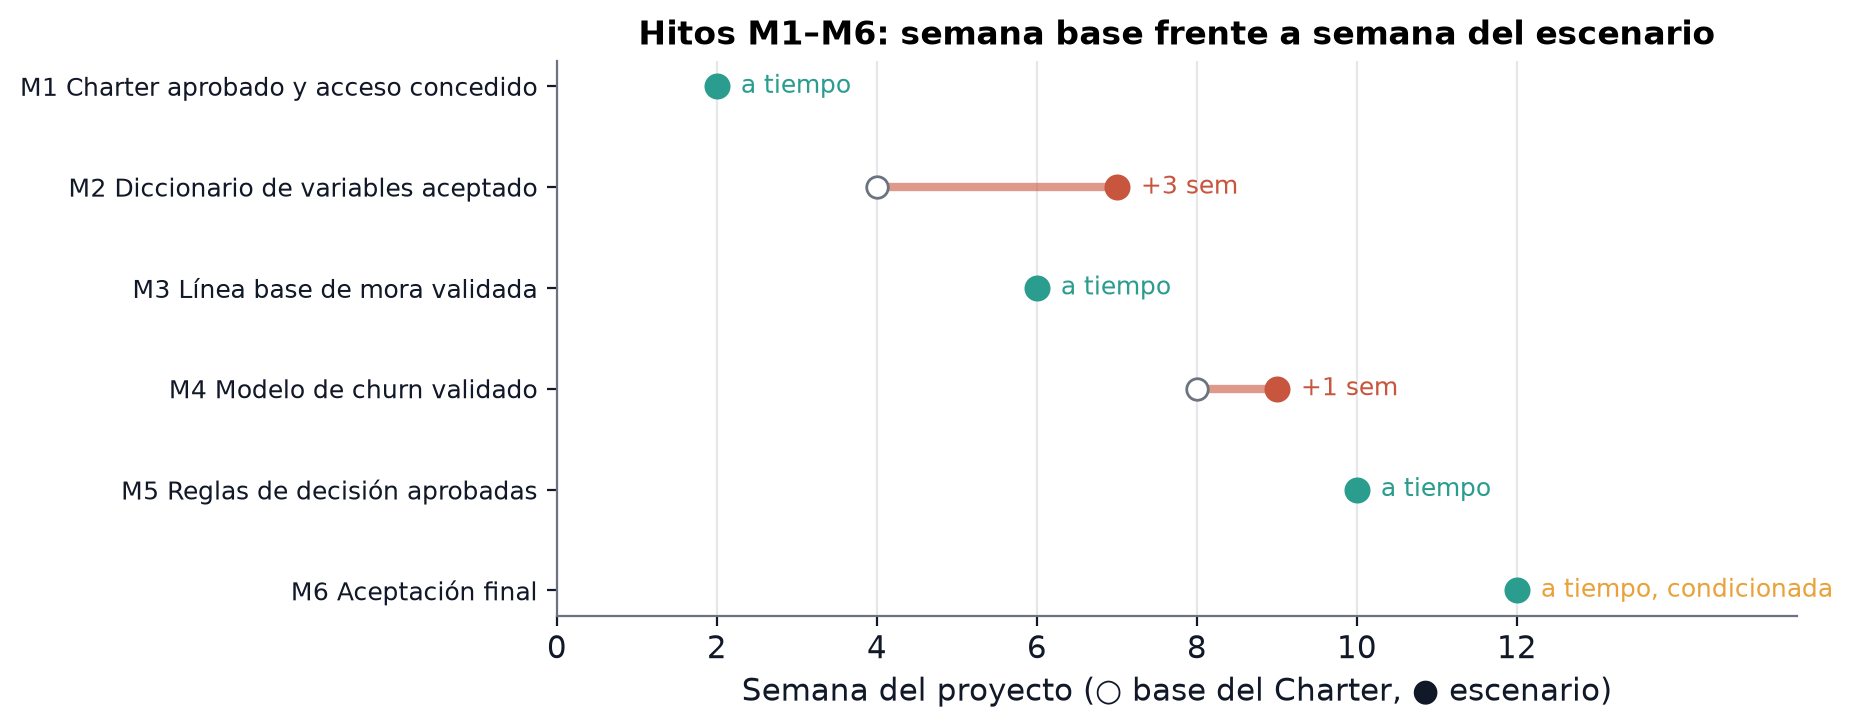
\includegraphics[width=0.78\linewidth]{../figures/milestones.png}\\[0.4em]
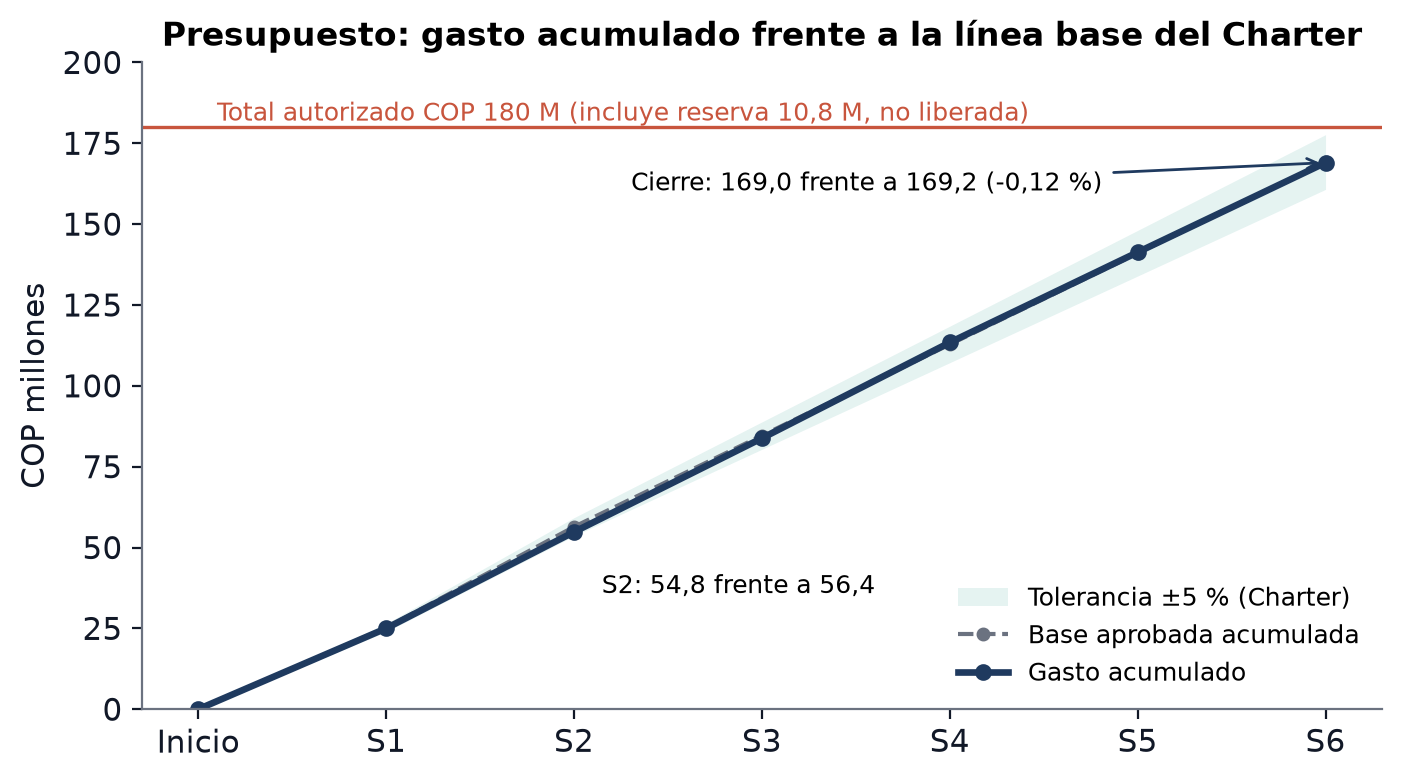
\includegraphics[width=0.66\linewidth]{../figures/budget_cumulative.png}
\caption{Hitos M1--M6 (semana base y semana del escenario) y gasto acumulado frente a la base del Charter}
\end{figure}

\begin{table}[h]
\caption{Registro de hitos}\label{tab:ms}
\scriptsize
\begin{tabularx}{\linewidth}{l p{2.6cm} l r r r X X}
\toprule
\textbf{Hito} & \textbf{Nombre} & \textbf{Obj.} & \textbf{Base} & \textbf{Esc.} & \textbf{Desv.} & \textbf{Condición} & \textbf{Evidencia} \\
\midrule
M1 & Charter aprobado y acceso concedido & O5 & 2 & 2 & 0 & Cumplido & US-01 y US-02 (S1); acuerdo Ley 1581 \\
M2 & Diccionario de variables aceptado & O1 O2 & 4 & 7 & +3 & Cumplido con retraso & T-05.2 (S2) y T-08.1 (S4): faltaban las variables de churn por el bloqueo de T-05.5 \\
M3 & Línea base de mora validada & O1 & 6 & 6 & 0 & Cumplido en el escenario; validación con datos reales pendiente & AUC fuera de tiempo del prototipo 0,7959 (30 d) y 0,7884 (60 d), PR \#17 \\
M4 & Modelo de churn validado & O2 & 8 & 9 & +1 & Cumplido con retraso en el escenario; validación con datos reales pendiente & Recall del prototipo 0,6203 al umbral 0,13, PR \#17 \\
M5 & Reglas de decisión aprobadas & O3 & 10 & 10 & 0 & Aprobación de Finanzas en el escenario; aprobación real pendiente & Matriz de costos y umbrales en src/finbank/pilot.py \\
M6 & Aceptación final & O4 O5 & 12 & 12 & 0 & Condicionada: firma del acta pendiente de la auditoría de protección de datos & docs/corte3/TRANSFERENCIA.md, PR \#20 \\
\bottomrule
\end{tabularx}

\end{table}

\textbf{Cronograma.} La desviación del hito final es de 0 semanas (0\,\% de 12 semanas). Los retrasos de M2 (+3) y M4 (+1) se absorbieron sin mover M3, M5 ni M6. M6 está \emph{condicionado}: la fecha se cumple, pero la aceptación real sigue pendiente.

\textbf{Presupuesto.} La desviación acumulada se calcula como $(\text{gasto acumulado} - \text{base acumulada}) / \text{base acumulada}$. La base del sprint $k$ es la planeación por rubro del Charter, y la reserva no se asigna a ningún sprint. Al cierre de S5 la desviación era \DesvScinco{} y el pronóstico al inicio de S6 (gasto real S1--S5 más la base de S6) era COP \EACSseis{} millones. El cierre real fue COP \GastoTotal{} millones (\DesvCosto). Por rubro, Gestión y gobierno superó su base un 4,8\,\% por las escalaciones y la auditoría, y Validación y documentación quedó por debajo. La compensación entre rubros no requiere liberar la reserva, pero el patrocinador debe conocerla. Del sobre autorizado quedan COP \NoEjecutado{} millones sin ejecutar, incluida la reserva completa.

\begin{table}[h]
\caption{Base y gasto por sprint (COP millones)}
\footnotesize
\begin{tabularx}{\linewidth}{l r r r r r X}
\toprule
\textbf{Sprint} & \textbf{Base} & \textbf{Gasto} & \textbf{Base acum.} & \textbf{Gasto acum.} & \textbf{Desv. acum.} & \textbf{Rótulo} \\
\midrule
S1 & 25,2 & 25,0 & 25,2 & 25,0 & -0,79 \% & Antecedente \\
S2 & 31,2 & 29,8 & 56,4 & 54,8 & -2,84 \% & Antecedente \\
S3 & 28,2 & 29,0 & 84,6 & 83,8 & -0,95 \% & Reconstrucción C3 \\
S4 & 28,2 & 29,6 & 112,8 & 113,4 & 0,53 \% & Reconstrucción C3 \\
S5 & 28,2 & 27,9 & 141,0 & 141,3 & 0,21 \% & Reconstrucción C3 \\
S6 & 28,2 & 27,7 & 169,2 & 169,0 & -0,12 \% & Simulación C3 \\
\textbf{Total} & \textbf{169,2} & \textbf{169,0} &  &  & \textbf{-0,12 \%} &  \\
\bottomrule
\end{tabularx}

\vspace{0.6em}
\caption{Base y gasto por rubro del Charter}
\footnotesize
\begin{tabularx}{\linewidth}{X r r r}
\toprule
\textbf{Rubro del Charter (COP millones)} & \textbf{Base} & \textbf{Gasto} & \textbf{Desviación} \\
\midrule
Gestión y gobierno & 27,0 & 28,3 & 4,8 \% \\
Ingeniería de datos & 45,0 & 45,1 & 0,2 \% \\
Modelado predictivo & 54,0 & 54,3 & 0,6 \% \\
Validación y documentación & 25,2 & 22,9 & -9,1 \% \\
Piloto, capacitación y transferencia & 18,0 & 18,4 & 2,2 \% \\
Reserva de contingencia (no asignada a sprints) & 10,8 & 0,0 & No liberada \\
\textbf{Total autorizado} & \textbf{180,0} & \textbf{169,0} & \textbf{No ejecutado: 11,0} \\
\bottomrule
\end{tabularx}

\end{table}

% ------------------------------------------------------------------ 9
\section{Resultados técnicos del piloto}

Los resultados de esta sección los produce el código del repositorio (commit \texttt{\SHA}) con datos sintéticos y semillas fijas \rot{Verificable}. Prueban que el método funciona de punta a punta. \textbf{No son una validación con datos de FinBank.} La validación fuera de tiempo usa una cohorte sintética independiente (\MuestraOOT{} clientes con observación, tasa de mora a 30 días de \TasaMora) que hace las veces de cohorte posterior.

\begin{table}[h]
\caption{Métricas del prototipo (\texttt{pilot\_metrics.csv})}\label{tab:pilot}
\footnotesize
\begin{tabularx}{\linewidth}{X r l r}
\toprule
\textbf{Métrica (prototipo, datos sintéticos)} & \textbf{Valor} & \textbf{Meta} & \textbf{n} \\
\midrule
AUC fuera de tiempo, mora 30 d & 0,7959 & $\geq$ 0,75 & 4.691 \\
AUC fuera de tiempo, mora 60 d & 0,7884 & $\geq$ 0,75 & 4.691 \\
AUC fuera de tiempo, churn 3 meses & 0,7673 &  & 4.000 \\
Umbral operativo churn (mayor beneficio con recall $\geq$ 0,60) & 0,13 &  & 4.000 \\
Recall churn, umbral operativo & 0,6203 & $\geq$ 0,60 & 4.000 \\
Precisión churn, umbral operativo & 0,2232 &  & 4.000 \\
Beneficio neto churn, umbral operativo (COP) & 11.550.000 &  & 4.000 \\
Umbral churn de solo costo & 0,21 &  & 4.000 \\
Recall churn, umbral de solo costo & 0,4094 & $\geq$ 0,60 & 4.000 \\
Precisión churn, umbral de solo costo & 0,3102 &  & 4.000 \\
Beneficio neto churn, umbral de solo costo (COP) & 20.055.000 &  & 4.000 \\
Umbral de mora (máximo beneficio) & 0,09 &  & 4.681 \\
\bottomrule
\end{tabularx}

\end{table}

En el segmento controlado (región andina), la lista semanal de alerta temprana marca \EWFlag{} de \EWTotal{} clientes de crédito para contacto de Cobranza (umbral \CorteMora), y la lista de churn propone \ChurnFlag{} de \ChurnTotal{} clientes preferenciales para una oferta de retención. Ambas listas usan un identificador seudonimizado (SHA-256 con sal), sin columnas personales.

\begin{figure}[h]
\centering
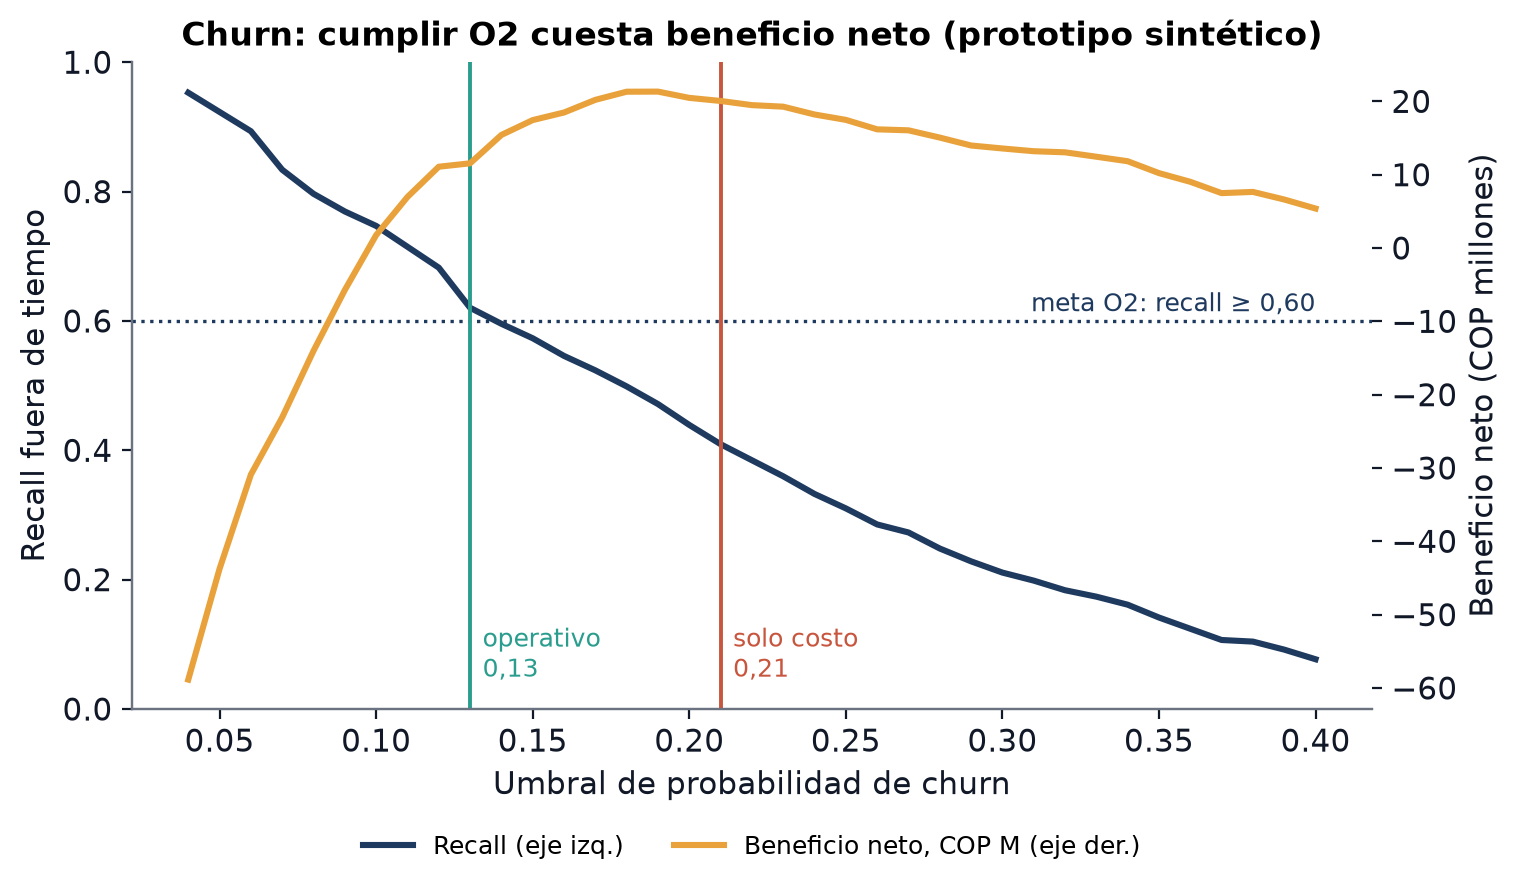
\includegraphics[width=0.49\linewidth]{../figures/churn_tradeoff.png}\hfill
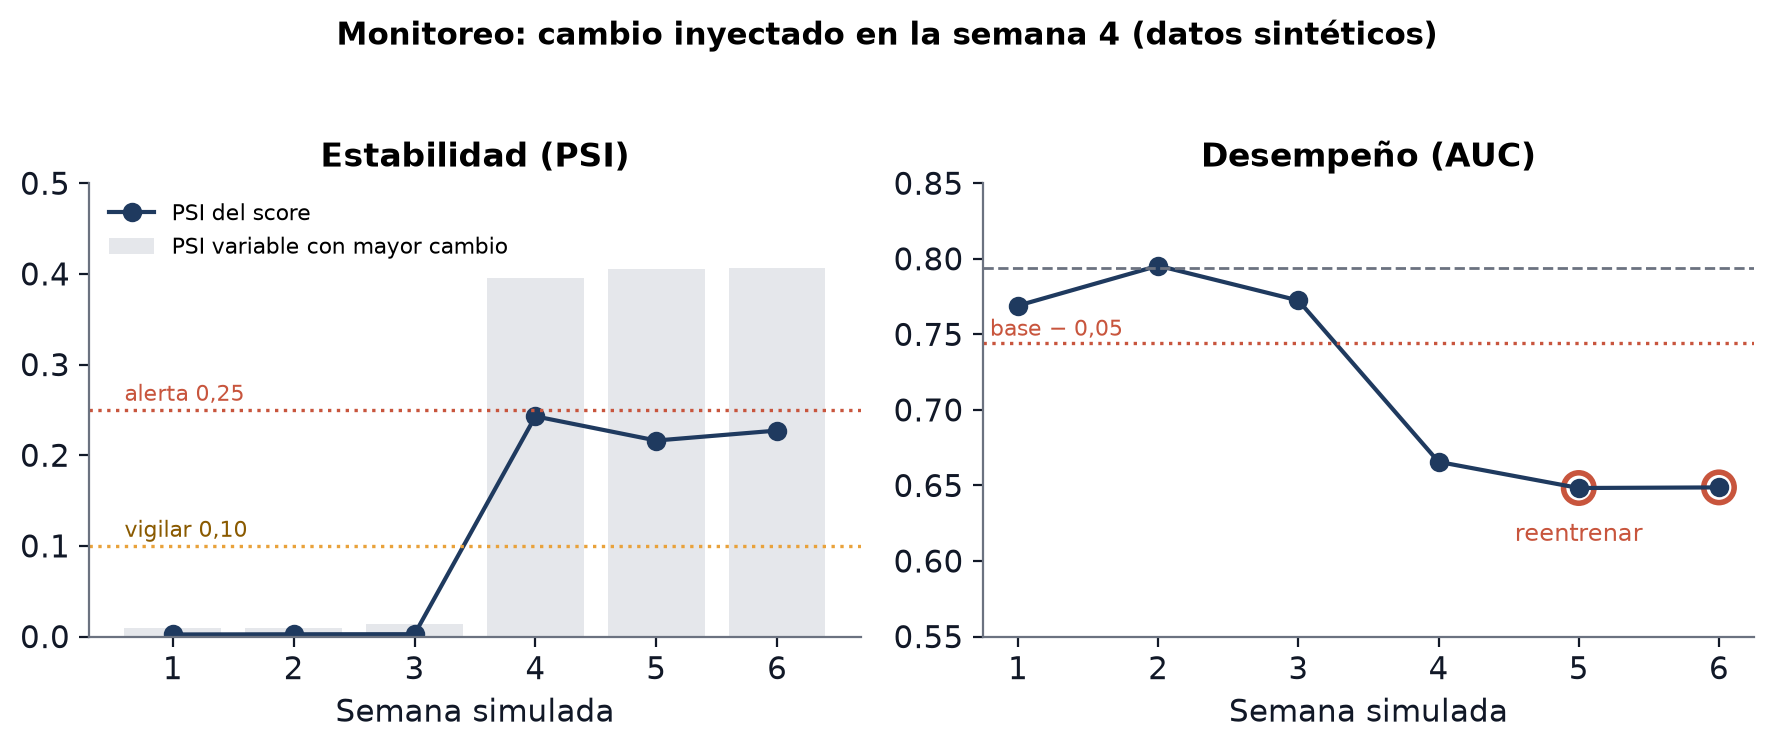
\includegraphics[width=0.49\linewidth]{../figures/monitoring.png}
\caption{Izquierda: el umbral de máximo beneficio (\CorteCosto) incumple O2; el umbral operativo (\CorteOp) lo cumple a cambio de COP \BenefDif{} M de beneficio neto. Derecha: el monitoreo detecta el cambio inyectado en la semana \SemAlerta{} (PSI de bureau\_score \PSIbureau) y marca reentrenamiento en la semana \SemReentreno{} (AUC \AUCsemReentreno{} frente a la base \AUCbase).}
\end{figure}

% ------------------------------------------------------------------ 10
\section{Retrospectiva, lecciones y acciones}

\begin{table}[h]
\caption{Acciones de mejora con responsable y seguimiento (S1--S6)}\label{tab:retro}
\footnotesize
\begin{tabularx}{\linewidth}{l X l l p{3.2cm}}
\toprule
\textbf{De} & \textbf{Acción de mejora} & \textbf{Resp.} & \textbf{Seguimiento} & \textbf{Estado} \\
\midrule
S1 & La DoD exige pruebas en verde y PR aprobado por un par; repositorio con CI & Oscar & S2 D1 & Hecha \\
S1 & Al menos dos sesiones de pairing por sprint registradas en la bitácora XP & Rafael & S2 & Hecha \\
S2 & Compromiso de S3 limitado a 16 puntos & Rafael & Planning S3 & Hecha \\
S2 & Definition of Ready: ninguna dependencia externa sin conceder entra al sprint & Oscar & Planning S3 & Hecha: dejó T-05.5 fuera de S3 \\
S2 & El Scrum Master escala impedimentos en menos de 24 horas & Oscar & S3-S6 & Hecha: escalación en S6 D4 \\
S4 & Las historias con ventana de observación se dividen por madurez del dato (US-08a y US-08b) & Rafael & Planning S5 & Hecha \\
S6 & Pedir la auditoría de protección de datos al inicio del sprint final y no en la Review & Daniel & Próximo proyecto & Abierta (lección) \\
S6 & Incluir la cuenta de servicio del ambiente de piloto en la Definition of Ready & Oscar & Próximo proyecto & Abierta (lección) \\
S6 & Separar en el tablero el Done del escenario y la aceptación real del negocio & Rafael & Transferencia a FinBank & Aplicada en el registro de aceptación \\
\bottomrule
\end{tabularx}

\end{table}

\textbf{Liderazgo y coordinación.}
\begin{itemize}
\item \textbf{Comprometer lo que se ha demostrado.} El exceso de compromiso de S2 (20 frente a 16) no se repitió. Desde S3 el compromiso se ató a la velocidad media y la variación entre sprints bajó.
\item \textbf{Escalar no es fallar.} Las dos escalaciones se hicieron en menos de 24 horas y protegieron el hito. El patrocinador conoció el problema antes de que se convirtiera en desviación.
\item \textbf{Separar el Done técnico de la aceptación del negocio.} El tablero de GitHub mide integración. El registro de aceptación mide lo que el cliente firmó. Mezclarlos habría mostrado un 100\,\% falso.
\item \textbf{El cumplimiento también tiene calendario.} La auditoría de protección de datos debió pedirse en la Planning de S6. Es la principal lección para el próximo proyecto.
\item \textbf{Roles.} El líder concentró la relación con el patrocinador y el presupuesto, el Product Owner las decisiones de orden y alcance, y el Scrum Master los impedimentos y las reglas del tablero. Separar los roles evitó que una sola persona decidiera alcance y plazo a la vez.
\end{itemize}

% ------------------------------------------------------------------ 11
\section{Decisión de cierre y transferencia}

\begin{tcolorbox}[colback=teal!6,colframe=teal!60,boxrule=0.5pt,arc=1mm]
\textbf{Decisión del patrocinador en la Review de S6} \rot{Simulación C3}: \textbf{cierre con transferencia condicionada.} Se aceptan los entregables de M3--M5 y el piloto. La firma del acta (O4) queda sujeta a que el oficial de protección de datos cierre el hallazgo de la sal en 5 días hábiles, sin costo adicional y sin liberar la reserva. No hay extensión de plazo: el Charter exige una nueva autorización para cualquier extensión.
\end{tcolorbox}

\textbf{Lo que queda pendiente y quién puede resolverlo} (actos reales, no simulados):
\begin{enumerate}
\item Firma del acta de entrega: el patrocinador, después de la auditoría del oficial de protección de datos.
\item Aprobación de la regla de decisión de churn (prioridad de O2 sobre O3): Finanzas.
\item Validación de O1 y O2 con el extracto real de FinBank: VP de Riesgo y TI, siguiendo la sección 6 del runbook.
\item Aprobación e integración de los PR \#16--\#21: Daniel Martínez o Rafael Baracaldo, cada uno en los PR que no escribió.
\item Sustentación académica del 20 de noviembre de 2026: el equipo. Este informe no la da por realizada.
\end{enumerate}

\textbf{Paquete de transferencia}: \path{docs/corte3/TRANSFERENCIA.md} (inventario, capacitación, DoR y DoD, auditoría y acta) y \path{docs/corte3/RUNBOOK.md} (operación semanal, controles y acciones por caso).

% ------------------------------------------------------------------ 12
\section{Discrepancias y limitaciones}
\begin{itemize}
\item \textbf{Fecha del Charter.} El Charter tiene fecha de emisión de septiembre de 2026, pero la cronología simulada sitúa S1 entre el 10 y el 21 de agosto. Se conserva la cronología de los Cortes 1 y 2 y se registra la diferencia.
\item \textbf{Dos calendarios.} Las fechas del escenario (agosto a octubre de 2026, 12 semanas) no coinciden con las académicas: trabajo técnico en GitHub en octubre y noviembre, entrega el 18 de noviembre y sustentación el 20. Los commits llevan la fecha real.
\item \textbf{Roles.} El Charter nombra a Rafael como analista de negocio y a Oscar como facilitador Scrum. Desde el Corte 2, en Scrum, son Product Owner y Scrum Master. Daniel conserva el reporte formal al patrocinador.
\item \textbf{Datos sintéticos.} Las métricas de los modelos son del prototipo. El enunciado prohíbe inventar AUC o recall, así que no se reporta ninguna cifra de modelo que no produzca el código.
\item \textbf{Consigna.} El sitio oficial del Corte 3 incrusta la consigna en un recurso de Canva que no se pudo descargar en esta preparación. Los requisitos se tomaron de la comprobación previa (dos PDF para el 18 de noviembre y sustentación formal el 20) y de la clase grabada del 6 de noviembre (30 minutos de presentación y 5 de preguntas). El equipo debe contrastarlos con la consigna completa.
\item \textbf{Número de grupo.} No está confirmado, así que se usa el marcador \emph{GrupoX} en los nombres de archivo.
\end{itemize}

% ------------------------------------------------------------------ anexos
\clearpage
\appendix
\section*{Anexo A. Registro de aceptación}
\addcontentsline{toc}{section}{Anexo A}
\scriptsize
\begin{tabularx}{\linewidth}{l X p{2.6cm} p{3.1cm} p{2.6cm}}
\toprule
\textbf{Ítem} & \textbf{Criterio} & \textbf{Escenario} & \textbf{Estado real} & \textbf{Quién lo resuelve} \\
\midrule
S6-01 & Lista semanal seudonimizada sin columnas personales & Cumple (S6 D8) & Integración en main pendiente de aprobación del PR & Revisor del PR (Daniel o Rafael) \\
S6-01 & Métricas rotuladas como prototipo sintético & Cumple & Validación con datos de FinBank pendiente & VP de Riesgo y TI con el extracto real \\
S6-01 & Dos corridas idénticas & Cumple & Verificado en CI & — \\
S6-01 & Validación de Cobranza contra el proceso operativo & Cumple (escenario S6 D8) & Pendiente: no hubo sesión real con Cobranza & Gerencia de Cobranza \\
S6-02 & Bandas de PSI estable / vigilar / alerta & Cumple (S6 D6) & Integración en main pendiente de aprobación del PR & Revisor del PR \\
S6-02 & Reentrenamiento tras 2 semanas con caída > 0,05 & Cumple & Integración en main pendiente de aprobación del PR & Revisor del PR \\
S6-02 & Detección del cambio inyectado & Cumple & Verificado en ejecución local y CI & — \\
S6-03 & Runbook ejecutable en copia limpia & Cumple (S6 D4) & Falta ejecución por un analista de FinBank & Analista de Riesgo en la capacitación real \\
S6-03 & Acción, rol y plazo por caso & Cumple & Integración en main pendiente de aprobación del PR & Revisor del PR \\
S6-04 & Inventario con ubicación y responsable & Cumple & Integración en main pendiente de aprobación del PR & Revisor del PR \\
S6-04 & Capacitación con registro de asistentes & Cumple (escenario S6 D8) & Pendiente: la sesión real no ocurrió & VP de Riesgo (convoca) y equipo DataForge \\
S6-04 & Acta firmable tras la auditoría de protección de datos & No cumple: hallazgo de la sal (S6 D10) & Pendiente & Oficial de protección de datos y luego el patrocinador \\
S6-05 & Base aprobada, gasto, pronóstico y reserva separados & Cumple (S6 D9) & Integración en main pendiente de aprobación del PR & Revisor del PR \\
S6-05 & Hitos M1-M6 con desviación y evidencia & Cumple & Integración en main pendiente de aprobación del PR & Revisor del PR \\
O1 & AUC $\geq$ 0,75 fuera de tiempo & Cumple en el prototipo: 0,7959 (30 d), 0,7884 (60 d) & Pendiente con datos reales & VP de Riesgo con el extracto real \\
O2 & Recall $\geq$ 0,60 al umbral operativo & Cumple en el prototipo: 0,6203 al umbral 0,13 & Pendiente con datos reales & VP de Riesgo y Retención \\
O3 & Matriz de costos y umbral aprobados por Finanzas & Aprobado en el escenario (Review S5) & Pendiente: aprobación real de Finanzas & Finanzas \\
O4 & Aceptación del paquete de transferencia por el patrocinador & Condicionada (Review S6) & Pendiente: firma real & Patrocinador \\
O5 & Desviación de costo y cronograma $\leq$ 5 \% & Cumple: costo -0,12 \%, hito final en la semana 12 & Cifras del escenario; sin registro contable real & Patrocinador y Finanzas \\
C3-00 & Dos PDF y sustentación & PDF generados en docs/corte3 & Entrega 18-nov-2026 y sustentación 20-nov-2026 pendientes & Equipo DataForge por el canal académico \\
\bottomrule
\end{tabularx}


\section*{Anexo B. Reproducción}
Desde una copia limpia del repositorio (\repo), en la rama \texttt{\Rama} (commit \texttt{\SHA}, generado el \Generado, Python \PyVer):
\begin{verbatim}
pip install -r requirements.txt -r requirements-corte3.txt
pytest -v                                  # pruebas
python scripts/run_pipeline.py             # incremento del Corte 2
python scripts/run_pilot.py                # piloto S6-01
python scripts/run_monitoring.py           # monitoreo S6-02
python scripts/github_snapshot.py          # tablero y bitácora desde GitHub
python scripts/build_corte3.py             # figuras, informe, PPTX, PDF y guion
\end{verbatim}
Resultado registrado en esta compilación: \textbf{\Tests{} pruebas en verde}. Las salidas completas están en \texttt{docs/corte3/evidence/}.

\begin{table}[h]
\caption{Detalle del monitoreo semanal (\texttt{monitoring\_report.csv})}
\footnotesize
\begin{tabularx}{\linewidth}{r r l X r r r l}
\toprule
\textbf{Sem.} & \textbf{PSI score} & \textbf{Estado} & \textbf{Variable con mayor PSI} & \textbf{PSI var.} & \textbf{AUC 30 d} & \textbf{Caída} & \textbf{Reentrenar} \\
\midrule
1 & 0,002 & estable & interest\_\allowbreak{}rate & 0,009 & 0,769 & 0,025 & no \\
2 & 0,003 & estable & monthly\_\allowbreak{}income & 0,009 & 0,795 & -0,001 & no \\
3 & 0,003 & estable & monthly\_\allowbreak{}income & 0,014 & 0,772 & 0,022 & no \\
4 & 0,243 & vigilar & bureau\_\allowbreak{}score & 0,396 & 0,666 & 0,129 & no \\
5 & 0,216 & vigilar & bureau\_\allowbreak{}score & 0,405 & 0,648 & 0,146 & sí \\
6 & 0,227 & vigilar & bureau\_\allowbreak{}score & 0,407 & 0,649 & 0,145 & sí \\
\bottomrule
\end{tabularx}

\end{table}

\section*{Anexo C. Índice de evidencias}
\small
\begin{tabularx}{\linewidth}{l X}
\toprule
\textbf{Evidencia} & \textbf{Ubicación} \\
\midrule
Datos fuente de tablas y gráficas & \texttt{docs/corte3/data/*.csv} (backlog, sprints, dailies, ítems de S6, hitos, presupuesto, aceptación, retro, bitácora GitHub) \\
Salidas de ejecución & \texttt{docs/corte3/evidence/} (pruebas, pipeline, piloto, monitoreo) \\
Tablero reproducible & \texttt{docs/corte3/TABLERO.md}; issues \href{https://github.com/OscarSantiagoMerino/DataForge-Consulting/issues?q=label\%3AC3}{label:C3} \\
Pull requests del Corte 3 & \href{https://github.com/OscarSantiagoMerino/DataForge-Consulting/pulls?q=label\%3AC3}{PR con label:C3} \\
Runbook y transferencia & \texttt{docs/corte3/RUNBOOK.md}, \texttt{docs/corte3/TRANSFERENCIA.md} \\
Presentación y guion & \texttt{docs/corte3/Presentacion\_FinBank\_GrupoX.pdf/.pptx}, \texttt{docs/corte3/Guion\_Sustentacion.md} \\
Índice navegable & \texttt{docs/corte3/README.md} \\
\bottomrule
\end{tabularx}

\end{document}
